%%%%%%%%%%%%%%%%%%%%%%%%%%%%%%%%%%%%%%%%%%%%%%%%%%%%%%%%%%%%%%%%%%%%%
% This is a LaTeX template for students
% working on Homework 6, Computer Architecture I, Spring, 2022.
% You SHALL NOT distribute this template.
%%%%%%%%%%%%%%%%%%%%%%%%%%%%%%%%%%%%%%%%%%%%%%%%%%%%%%%%%%%%%%%%%%%%%
\section{Oops \dots Too many bites (bytes)}
In this sections, we will review the implementation of caches and
replacement policies.

\begin{questions}

\question[15] Let's Draw It Out!

Sketch the organization of a \emph{four-way set associative} cache
with a cache block size of 16 bytes and a total size of 128 bytes.
Your sketch should have a style similar to Figure 1. The memory
addresses are 12-bit long.

In your sketch, the following components should be also presented.

\begin{enumerate}
    \item the width of set index, tag and data fields of memory
    addresses (3 points),
    \item logical components used for comparison and selection
    (2 points),
    \item the type of multiplexer (e.g. $2\rightarrow1$,
    $4\rightarrow1$, $8\rightarrow1$, $16\rightarrow1$, etc.)
    (1 point),
    \item the number of sets (1 point) , and,
    \item an implementation layout including wiring and placement
    of cache elements (8 points).
\end{enumerate}



{
    \begin{solution}
    % DRAWING BY HAND IS HIGHLY RECOMMENDED!
    % You are not recommended to draw it with LaTeX, as it will
    % take you TREMENDOUS time. Let's make our life more easier :)
    % So, please attach your figures in `img/` directory and use
    % \includegraphics{}
    % to display it here.

    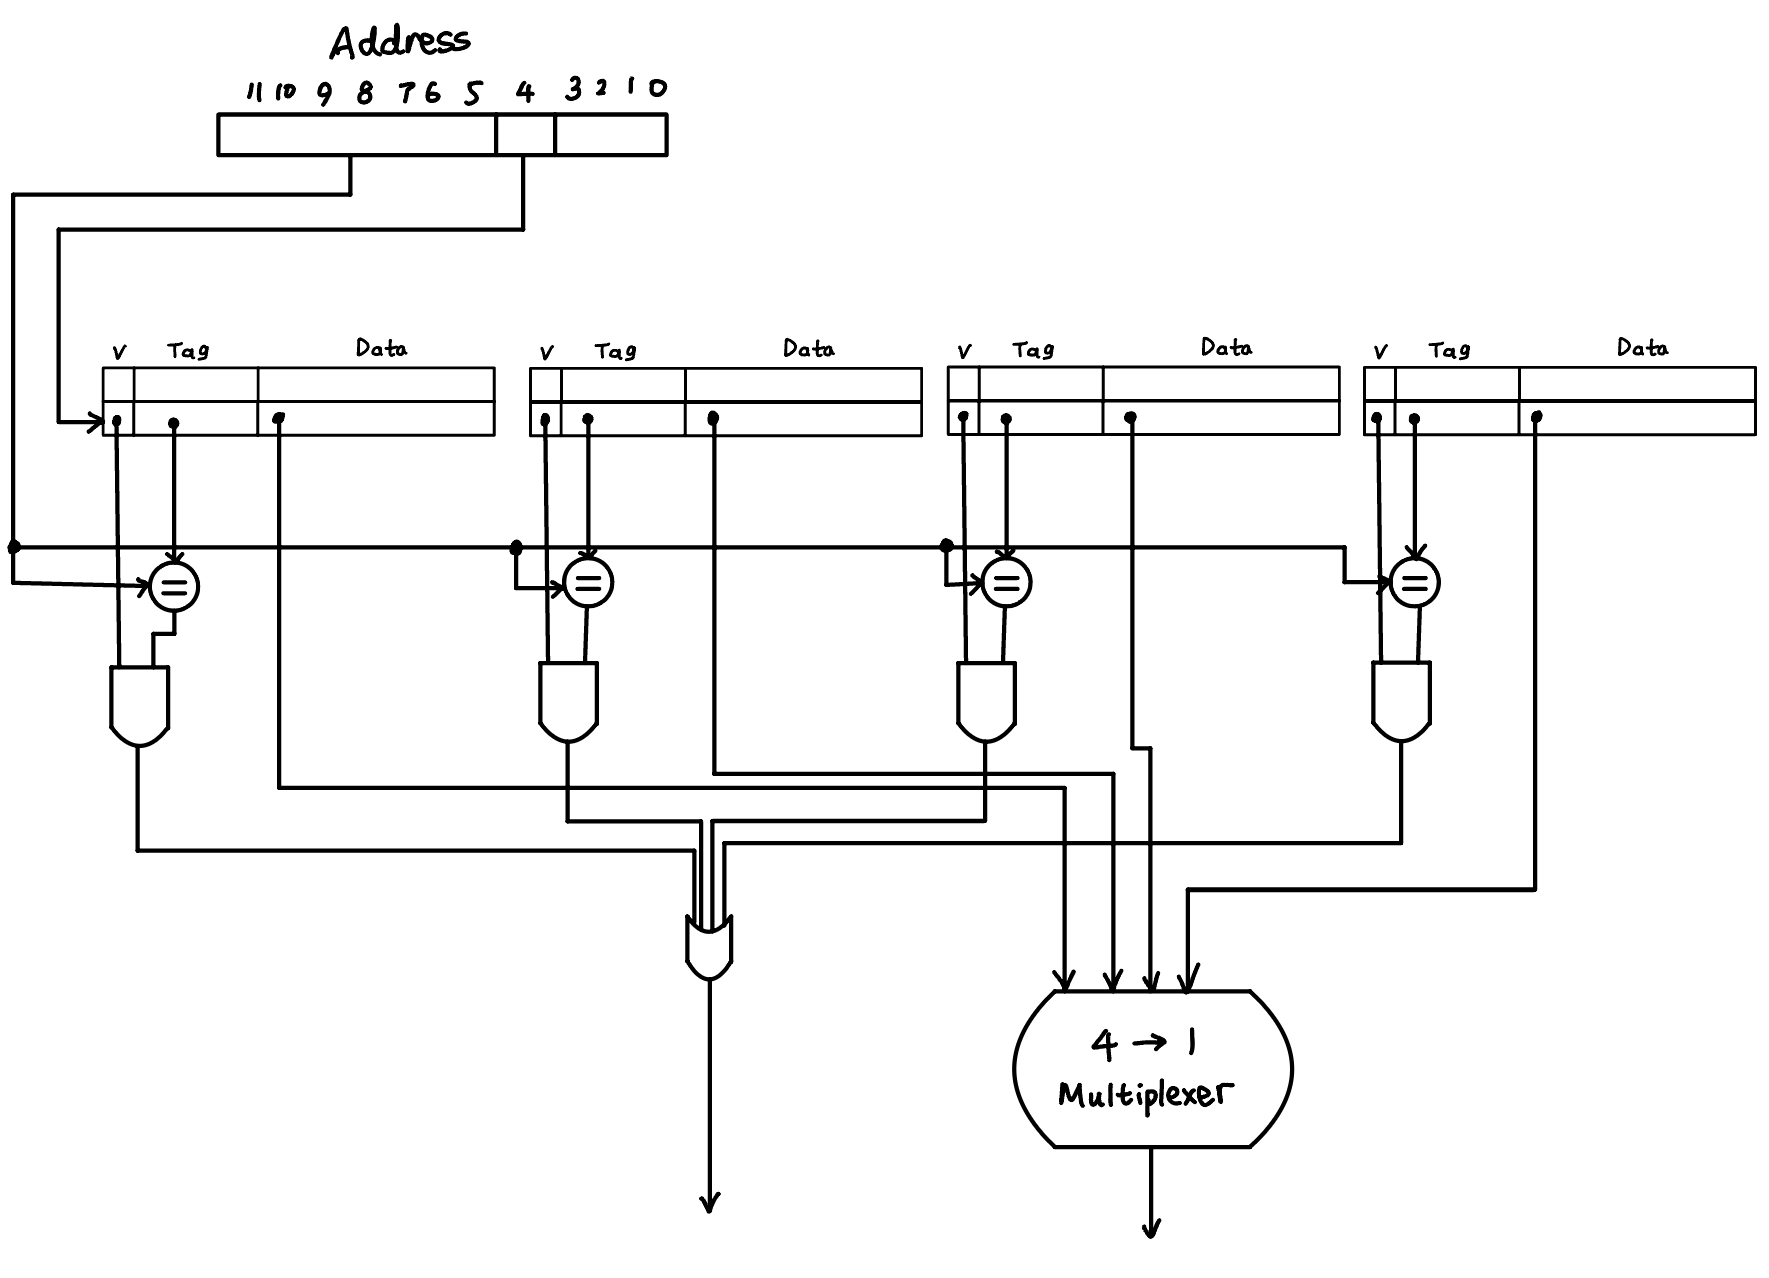
\includegraphics[scale=0.25]{q2.jpeg}

    \vspace{5in}
    \end{solution}
}
\newpage

In the following questions, we will examine how replacement policies
affect miss rate.

After the system is cold start, the address sequence of warm-up
accesses is:\\
\texttt{0x2A, 0x3C, 0x7D, 0xCE, 0x5B, 0x01, 0x2C, 0x1D, 0x9B, 0x3E}.

After all warm-up accesses are done, the address sequence of
follow-up accesses is: \\
\texttt{0x30, 0x40, 0x52, 0x44, 0x56, 0x48, 0x5A, 0x4C, 0x10, 0x3B,
0x5C, 0x30, 0x5E}.

\question[2] Which locality(s) can you observe in the follow-up
accesses?

{

    \begin{solution}
        Note: There may exist(s) one or more correct choice(s).\\
        \begin{oneparcheckboxes}
            \CorrectChoice Spatial locality
            \CorrectChoice Temporal locality
        \end{oneparcheckboxes}
    \end{solution}

}

\question[2] Assume \emph{Least Recently Used} (LRU) replacement
policy is applied. Circle out all access(es) with cache hit in
the follow-up accesses. \label{q:lru}

{
    \begin{solution}
        % Use \Circled{} to surround the access you want to choose.
        Circle the access(es) that meets a cache hit!
        (like this: \texttt{\Circled{0xFF}})\\
        \begin{center}
        \texttt{\Circled{0x30}, 0x40, \Circled{0x52}, \Circled{0x44}, \Circled{0x56}, \Circled{0x48}, \Circled{0x5A}, \Circled{0x4C}, \Circled{0x10},
        \Circled{0x3B}, \Circled{0x5C}, \Circled{0x30}, \Circled{0x5E}}.
        \end{center}
        \vspace{7px}
    \end{solution}
}

\question[2] Assume \emph{Most Recently Used} (MRU) replacement policy
is applied. Circle out all access(es) with cache hit in the follow-up
accesses. \label{q:mru}

{
    \begin{solution}
        % Use \Circled{} to surround the access you want to choose.
        Circle the access(es) that meets a cache hit!
        (like this: \texttt{\Circled{0xFF}})\\
        \begin{center}
        \texttt{\Circled{0x30}, 0x40, \Circled{0x52}, \Circled{0x44}, \Circled{0x56}, \Circled{0x48}, \Circled{0x5A}, \Circled{0x4C}, 0x10,
        \Circled{0x3B}, 0x5C, 0x30, 0x5E}.
        \end{center}
        \vspace{7px}
    \end{solution}
}

\question[6] 
The specification sheet of the system is given below. What is the
Average Memory Access Time (AMAT) of memory accesses in the question
\ref{q:lru} and \ref{q:mru}? Please give your answer in nanosecond 
(ns). You shall have the formula, the unit of results and the
deriving procedure presented in your answer. (Note: A 1 gigahertz
(GHz) processor ticks a cycle for each 1 nanosecond)

\begin{table}[h]
    \centering
    \begin{tabular}{l l}
        \hline % ---------------------------------
        System Frequency           & 2 GHz      \\
        Cache Access Latency       & 2 Cycles   \\
        Main Memory Access Latency & 130 Cycles \\
        \hline % ---------------------------------
    \end{tabular}
    \caption{Specification Sheet}
    \label{tab:spec_sheet}
\end{table}

{
    \pagebreak
    \begin{solution}
        %%%%%%%%%%%%%% YOUR ANSWER HERE %%%%%%%%%%%%%%%%%%%%%%%%%

        In both problems, 

        Time for one clock cycle = 1 / System frequency = 0.5ns

        Hit time = Cache Access Latency = 2 Cycles = 1ns

        Miss Penalty = Main Memory Access Latency = 130 Cycles = 65ns

        \begin{enumerate}
            \item In problem 3, the Miss Rate is $1/13$
            
            AMAT = hit time + miss rate $\times$ miss penalty

            \ \ \ \ \ \ \ \ \ \ = 1 + $\frac{1}{13} \times $ 65

            \ \ \ \ \ \ \ \ \ \ = 6ns

            \item In problem 4, the Miss Rate is $5/13$
            
            AMAT = hit time + miss rate $\times$ miss penalty

            \ \ \ \ \ \ \ \ \ \ = 1 + $\frac{5}{13} \times $ 65

            \ \ \ \ \ \ \ \ \ \ = 26ns

        \end{enumerate}

        %%%%%%%%%%%%%%%%%%%%%%%%%%%%%%%%%%%%%%%%%%%%%%%%%%%%%%%%%
        \vspace{1in}
    \end{solution}
}


\end{questions}
